\documentclass{beamer}

% Theme selection
\usetheme{Madrid} % Choose a theme that suits your presentation style

% Packages
\usepackage{graphicx} % For including images
\usepackage{amsmath} % For mathematical equations
\usepackage{booktabs} % For better table formatting

% Title and author information
\title{Field-Oriented Control of Induction Motors: Enhanced Performance and Efficiency}
\author{[Your Names]}
\institute{Rajalakshmi Engineering College}
\date{May 2, 2024}

\begin{document}

\begin{frame}
  \titlepage
\end{frame}

\begin{frame}{Introduction}
  \begin{itemize}
    \item Induction motors are widely used in industry.
    \item Precise control is crucial for high-performance applications.
    \item Traditional scalar control methods have limitations.
    \item Field-Oriented Control (FOC) offers superior performance.
  \end{itemize}
\end{frame}

\begin{frame}{Advantages of FOC}
  \begin{itemize}
    \item Precise Torque and Speed Control
    \item Improved Efficiency
    \item Enhanced Dynamic Response
    \item Reduced Motor Stress
  \end{itemize}
\end{frame}

\begin{frame}{FOC Block Diagram}
  \begin{figure}
    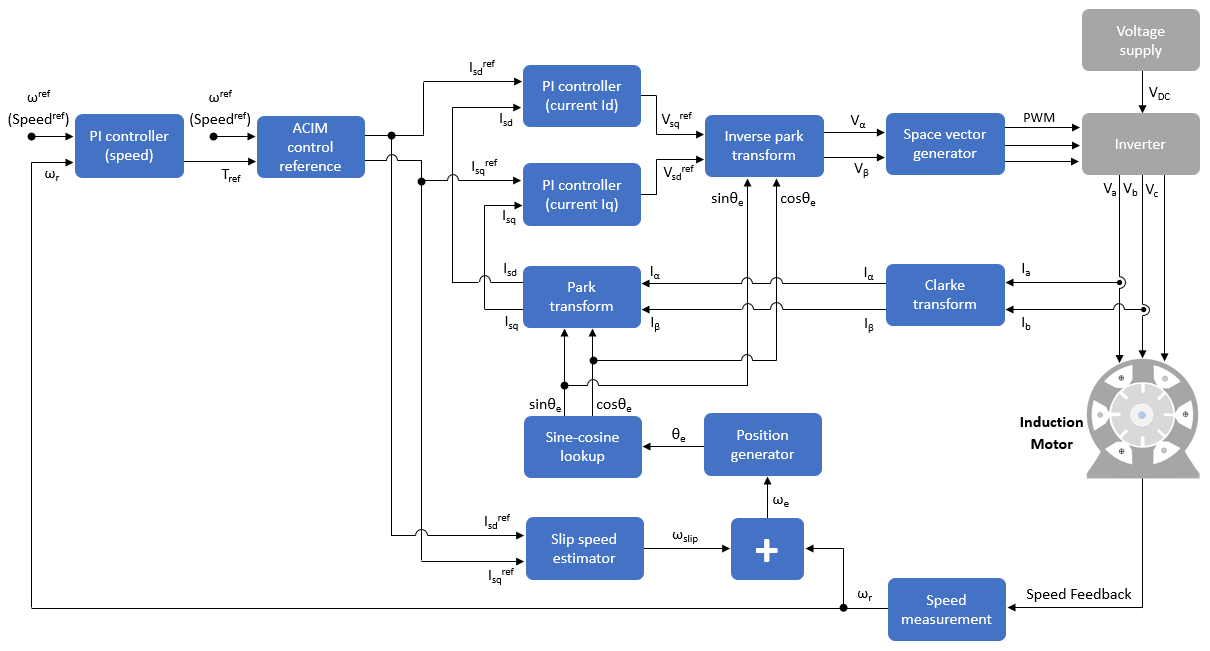
\includegraphics[width=4in]{conference/blockDiagram.png} % Replace with your block diagram image
    \caption{FOC Block Diagram}
  \end{figure}
  \begin{itemize}
    \item Coordinate Transformations
    \item PI Controllers
    \item Inverse Transformations
    \item PWM Generation
  \end{itemize}
\end{frame}

\begin{frame}{Rotor Flux Angle Estimation}
  \begin{itemize}
    \item Accurate estimation is critical.
    \item Sensorless vs. Sensor-based methods
    \item Trade-offs: Cost vs. Accuracy
  \end{itemize}
\end{frame}

\begin{frame}{Project Overview}
  \begin{itemize}
    \item Simulation and comparison of FOC and V/f control
    \item Analysis of output filter (OTT filter) impact
    \item MATLAB/Simulink environment
  \end{itemize}
\end{frame}

\begin{frame}{MATLAB/Simulink Implementation}
  \begin{columns}
    \begin{column}{0.5\textwidth}
      \begin{figure}
        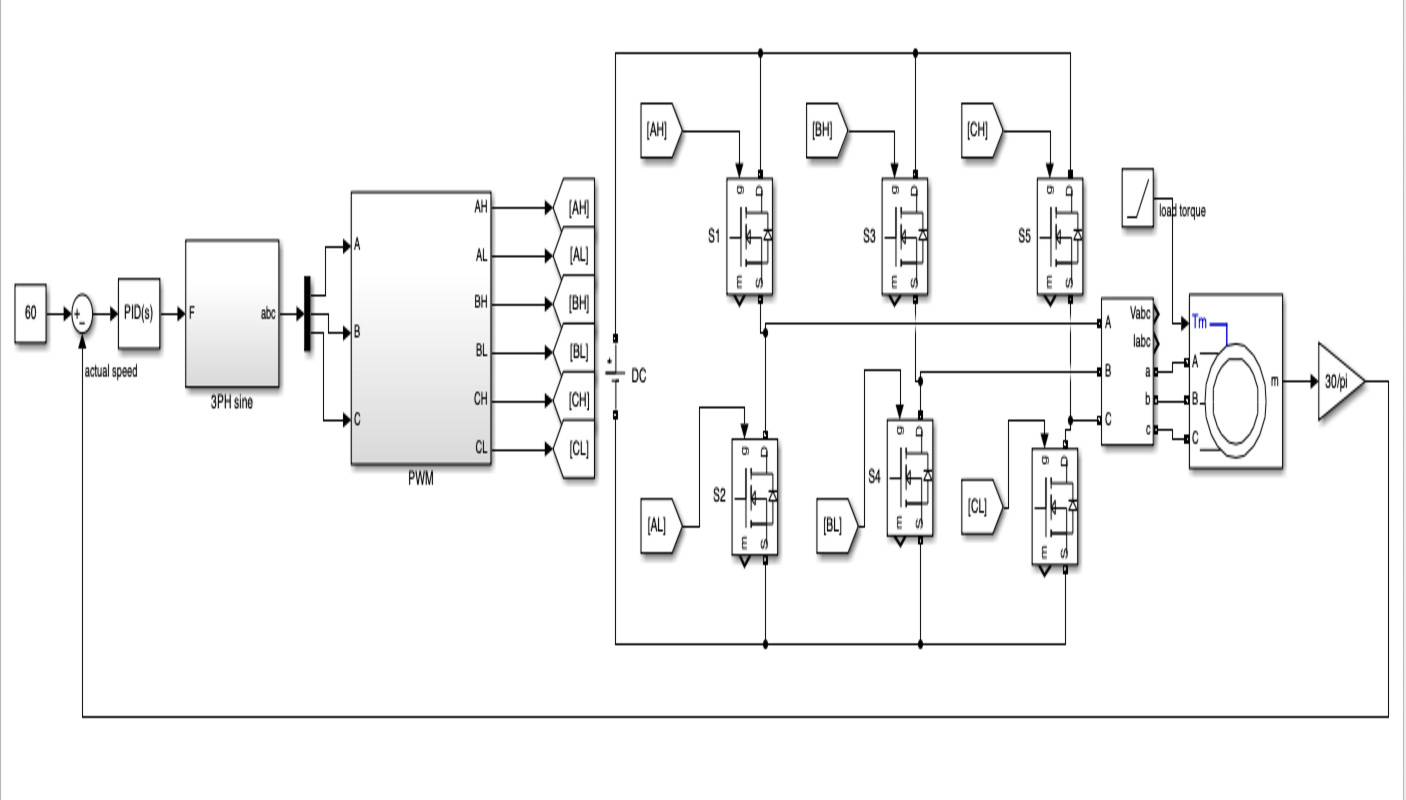
\includegraphics[width=4in]{conference/vfSimulation.png} % Replace with your V/f control Simulink image
        \caption{V/f Control Simulink Diagram}
      \end{figure}
    \end{column}
    \begin{column}{0.5\textwidth}
      \begin{figure}
        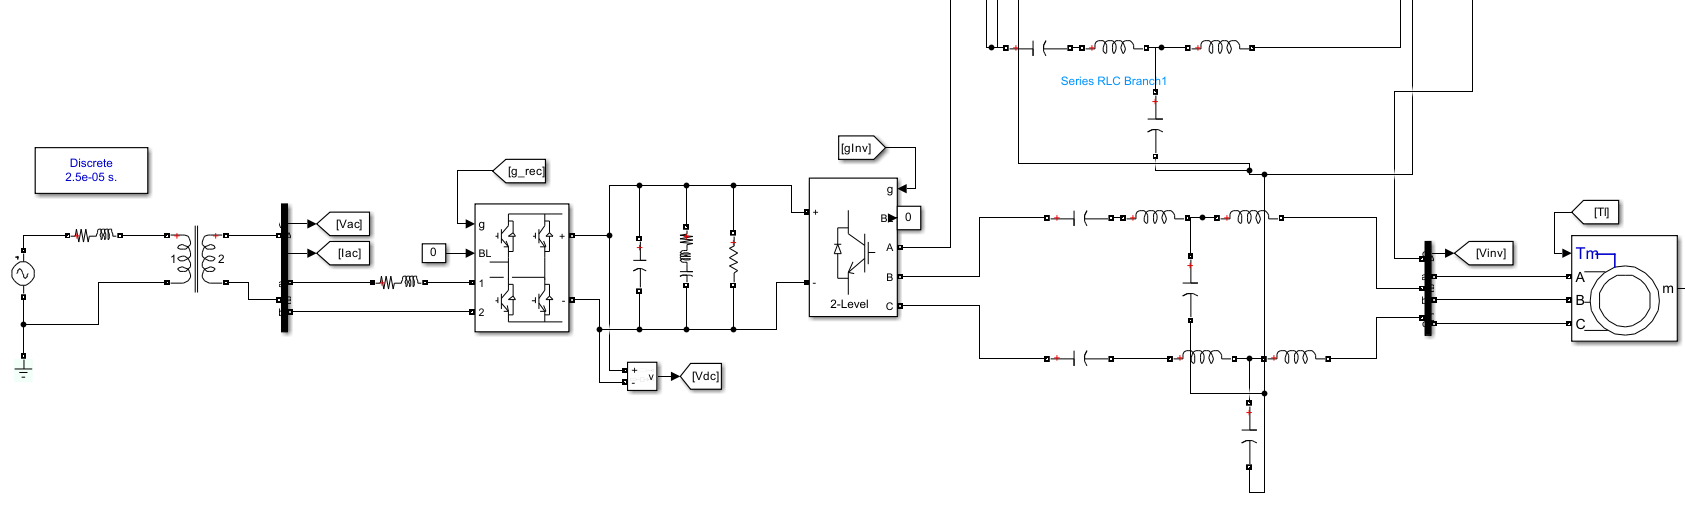
\includegraphics[width=4in]{conference/matlab.png} % Replace with your FOC Simulink image
        \caption{FOC with OTT Filter Simulink Diagram}
      \end{figure}
    \end{column}
  \end{columns}
\end{frame}

\begin{frame}{Performance Comparison: Speed Response}
  \begin{figure}
    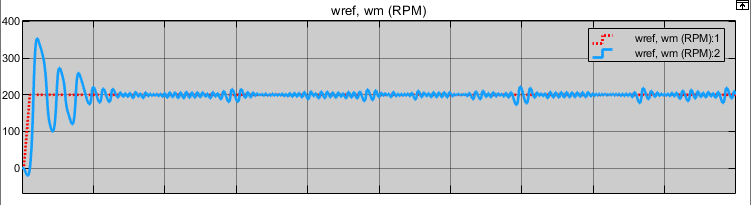
\includegraphics[width=4in]{conference/Speed_conf.png} % Replace with your speed response comparison graph
    \caption{Speed Response Comparison}
  \end{figure}
\end{frame}

\begin{frame}{Performance Comparison: Torque Response}
  \begin{figure}
    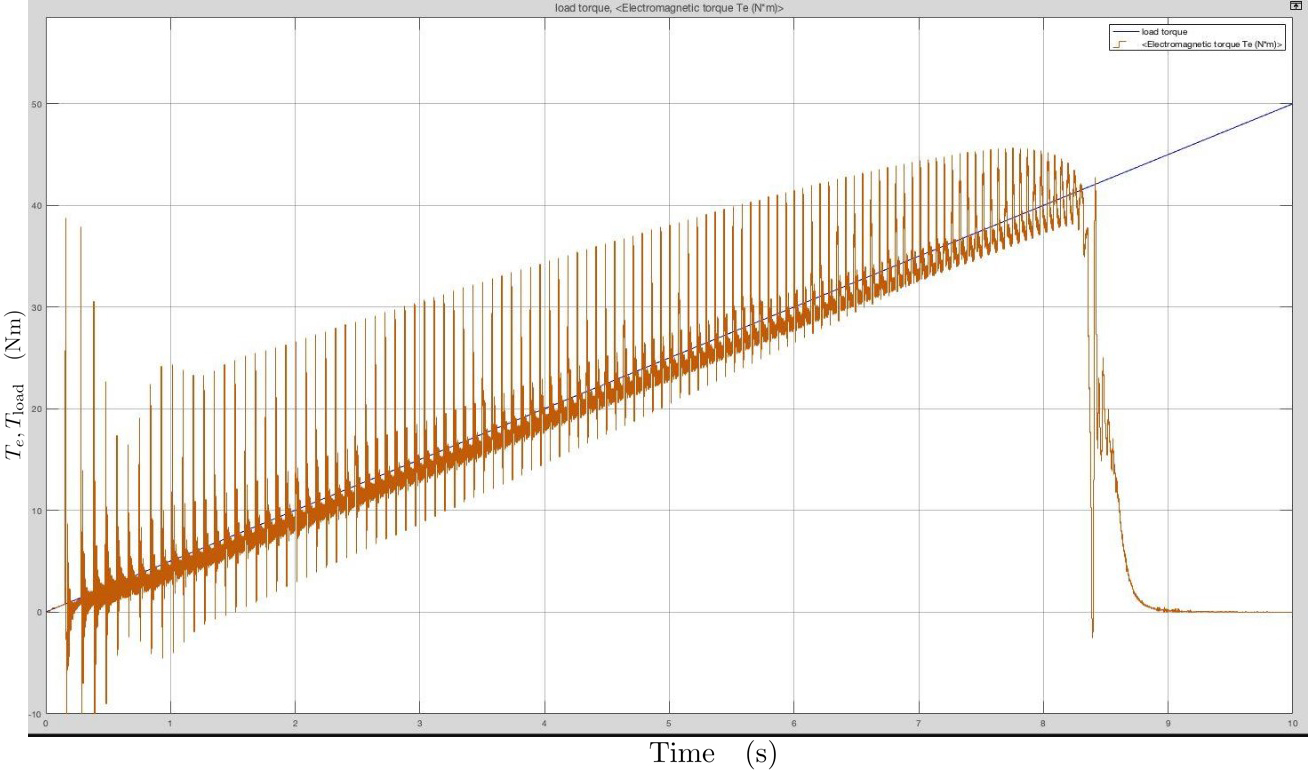
\includegraphics[width=4in]{conference/60rpmTorque.jpeg} % Replace with your torque response comparison graph
    \caption{Torque Response Comparison}
  \end{figure}
\end{frame}

\begin{frame}{Harmonic Distortion Analysis}
  \begin{figure}
    \includegraphics[width=4in]{placeholder_thd_comparison.png} % Replace with your THD comparison graph
    \caption{THD Comparison}
  \end{figure}
\end{frame}

\begin{frame}{Conclusion}
  \begin{itemize}
    \item FOC offers significant performance benefits.
    \item Simulation platform enables efficient design and analysis.
    \item Future work: Real-time implementation and sensor integration.
  \end{itemize}
\end{frame}

\begin{frame}{Applications of FOC}
  \begin{itemize}
    \item Electric Vehicles
    \item Robotics
    \item CNC Machines
    \item High-Performance Industrial Drives
  \end{itemize}
\end{frame}

\begin{frame}{Thank You \& Questions}
\end{frame}

\end{document}